The process of technical nuclear forensics includes the analysis and
interpretation of nuclear material to determine its history, whether that be
intercepted \gls{SNF}, \gls{UOC}, or the debris from an exploded nuclear
device. After the technical portion is complete, intelligence data is used
to aid in material attribution; this is the overall goal of nuclear forensics. 

After a nuclear incident, the material or debris is sampled and evaluated
through many techniques that provide the following information: material
structure, chemical and elemental compositions, and radioisotopic compositions
and/or ratios.  These measurements or ratios comprise the forensic signatures
of the sample in question. These signatures can be analyzed with specific
domain knowledge; for example, \gls{UOC} will have trace elements depending on
where it was mined from.  They can also be analyzed against a materials
reference database in the case of \gls{SNF}.

Measurement needs and techniques vary vastly depending on the material, as does
the type of signature. This study focuses on non-detonated materials,
specifically, \gls{SNF}. Tracing the source to an entity or state depends on
determining if some intercepted \gls{SNF} is from an undisclosed reactor or a
commercial fuel cycle. This can be done by following the steps shown in Figure
\ref{fig:rwforensics}.  First, select chemical and elemental signatures and
isotopic ratios are obtained, and these measurements are compared to those in
an existing forensics database of reference \gls{SNF}.  The signatures for
\gls{SNF} correlate to characteristics that can, in a best case scenario with a
reactor history database, point to the exact reactor from which the fuel was
intercepted.  The reactor parameters of interest are the reactor type, fuel
type, enrichment at beginning of irradiation, cooling time, and burnup
\cite{weber_2006, weber_2010, weber_2011}.

\begin{figure}[!tbh]
  \makebox[\textwidth][c]{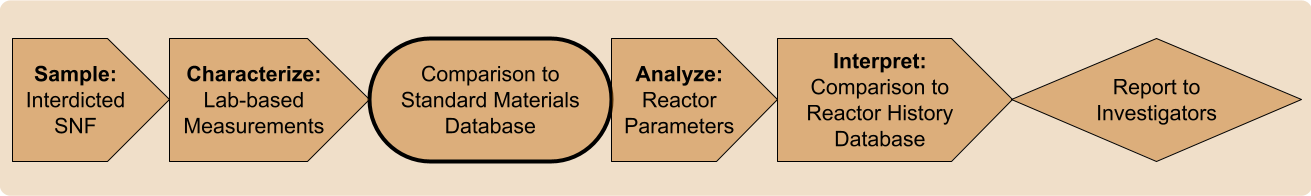
\includegraphics[width=\linewidth]{./chapters/intro/ForensicsWorkflow.png}}
  \caption{An example workflow for a nuclear forensics investigation.}
  \label{fig:rwforensics}
\end{figure}

The current and future work of this study are designed based on two primary
needs to bolster the \gls{US} nuclear forensics capability: post-incident rapid
characterization, and forensics database challenges and imperfection.  

First, our best measurement techniques cannot be available in an emergency
scenario, and fast measurements typically yield inaccurate results.  Currently,
both radiological measurements and mass spectrometry are used in nuclear
forensics exercises.  Because these techniques have a multitude of variants
within each category, there are differing levels of measurement uncertainties.
A lofty goal would be to develop methods that provide instantaneous
information, reliable enough to guide an investigation (e.g., within 24 hours).
In the case of \gls{SNF}, it takes weeks in a lab to measure isotopes via
advanced (cooled detector) gamma spectroscopy and mass spectrometry equipment.
A handheld detector that measures gamma spectra could provide the fast
measurements to calculate isotopic ratios for the above-mentioned fuel
parameters of interest.  However, while this nondestructive analysis is rapid,
it is also difficult to evaluate because of the presence of overlapping peaks
and the fact that uncertainties differ significantly because of the detector
response, environment, storage, electronics, etc. Broadly speaking, there is a
time/cost and information tradeoff: gamma spectra give less information at a
higher uncertainty than the near-perfect results of the destructive mass
spectrometry techniques used for characterization, such as inductively coupled
plasma mass spectrometry \cite{iaea_nf}.

Second, forensics databases present challenges; this is three-fold.  Because of
the values needed for material provenance, forensics databases are highly
multidimensional. Also because of the number of measurement types, the
forensics databases have inconsistent uncertainties or missing data entries
\cite{nf_missingdata}.  Thus, direct comparison between measurement results and
a database therefore may not yield accurate parameter predictions.
Furthermore, these databases are kept by individual countries, and the reactor
operation history information is well-guarded, so it may be difficult to study
\gls{SNM} from a country that has a different fuel cycle.  It is proposed that
using a statistical model generated using simulated \gls{SNF} may be able to
combat these issues; this is introduced next in Section \ref{sec:statscontrib}. 
